\apendice{Especificación de diseño}

\section{Introducción}
En esta sección se describen algunas características relacionadas con el diseño del proyecto.

\section{Diseño de datos}

\subsection{Sensores}
Para este proyecto era necesario la obtención dinámica de datos de sensores en tiempo real, para ello el cliente facilitó una serie de sensores que disponía en una bodega y almacenaba los datos en PRTG, los sensores en cuestión miden el consumo de la bomba de agua \ref{img_Consumo_Bomba_Agua}, la humedad en el ambiente \ref{mg_Humedad_Ambiente_PRTG}, la humedad en la parcela \ref{img_Humedad_Parcela_PRTG} y la presión de la tubería de agua.\ref{img_Presion_Tuberia_Agua_PRTG}



\begin{figure}[!h]
	\centering
	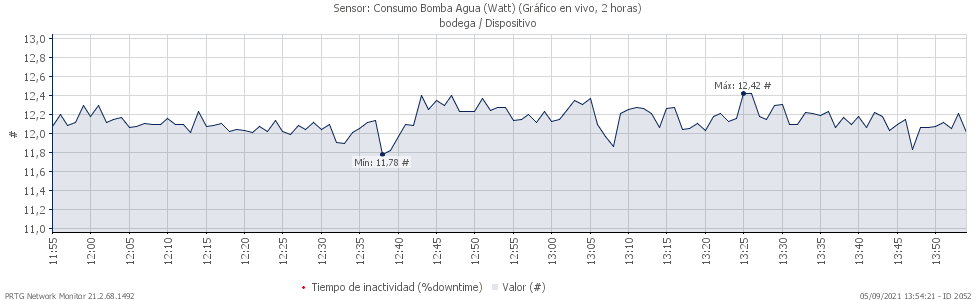
\includegraphics[width=0.95\textwidth]{img/img_PRTG_Consumo_bomba_agua.png}
	\caption{Sensor del consumo de la bomba de agua}
	\label{img_Consumo_Bomba_Agua}
\end{figure}

\begin{figure}[!h]
	\centering
	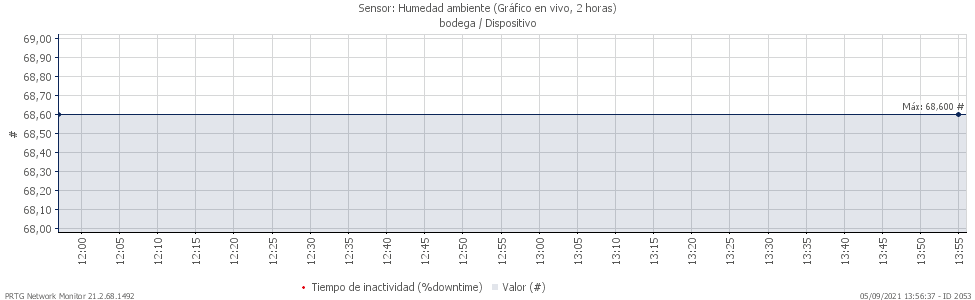
\includegraphics[width=0.95\textwidth]{img/img_PRTG_Humedad_ambiente.png}
	\caption{Sensor de la humedad en el ambiente}
	\label{mg_Humedad_Ambiente_PRTG}
\end{figure}

\begin{figure}[!h]
	\centering
	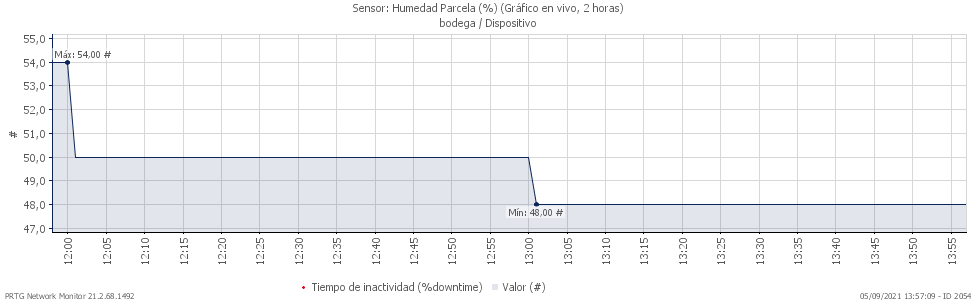
\includegraphics[width=0.95\textwidth]{img/img_PRTG_Humedad_parcela.png}
	\caption{Sensor de la humedad en la parcela}
	\label{img_Humedad_Parcela_PRTG}
\end{figure}

\begin{figure}[!h]
	\centering
	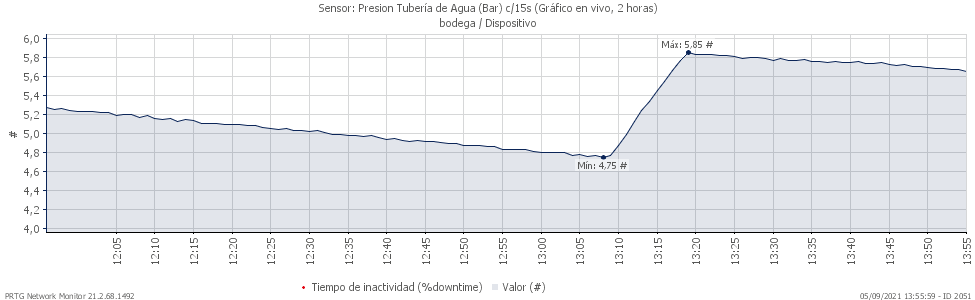
\includegraphics[width=0.95\textwidth]{img/img_PRTG_Presion_tuberia_agua.png}
	\caption{Sensor de la presión de la tubería de agua}
	\label{img_Presion_Tuberia_Agua_PRTG}
\end{figure}

\clearpage

\subsection{Base de datos}

Los datos de los sensores, una vez extraídos de PRTG, se almacenan en Elasticsearch, una base de datos NoSQL orientada a documentos. A diferencia de las bases de datos relacionales, esta no está estructurada en filas y columnas, Elasticsearch almacena cada registro junto a sus datos asociados en un único documento JSON \ref{json-linea-example} el cual es asociado a un index. Para ver más información sobre la indexación y la estructura de los ficheros consultar el manual de usuario en el anexo E.

\begin{listing}
\begin{minted}[frame=single,
               framesep=3mm,
               linenos=true,
               xleftmargin=21pt,
               tabsize=6]{js}

{
    "sensorId":"2051",
    "datetime":"27/07/2021 16:13:06",
    "reading": 
    {
        "Valor":4.6700,
        "Tiempo de ejecución":799.0000
    }
}
\end{minted}
\caption{ejemplo línea de un fichero JSON} 
\label{json-linea-example}
\end{listing}

\clearpage

\subsection{Diagrama de clases}
 A continuación, se mostrarán los diagramas de clase de la aplicación para facilitar el entendimiento de la estructura del sistema. En la figura \ref{img_diagrama_clases_modelo} se muestra las clases del paquete \textit{/Prediccion} en la cual se encuentra el modelo de aprendizaje y en la figura \ref{img_diagrama_clases_Utilidades} se representan las clases del paquete \textit{/Utilidades} y \textit{/Gestion\_datos} .
 
\begin{figure}[!h]
	\centering
	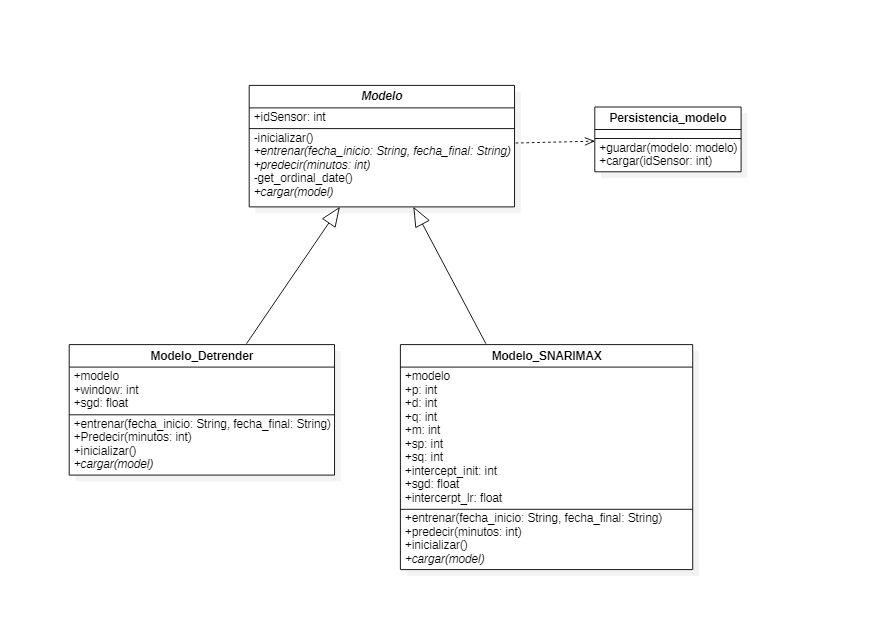
\includegraphics[width=1.1\textwidth]{img/img_diagrama_clases_modelo.png}
	\caption{Diagrama de clases paquete Predicción}
	\label{img_diagrama_clases_modelo}
\end{figure}

\begin{figure}[!h]
	\centering
	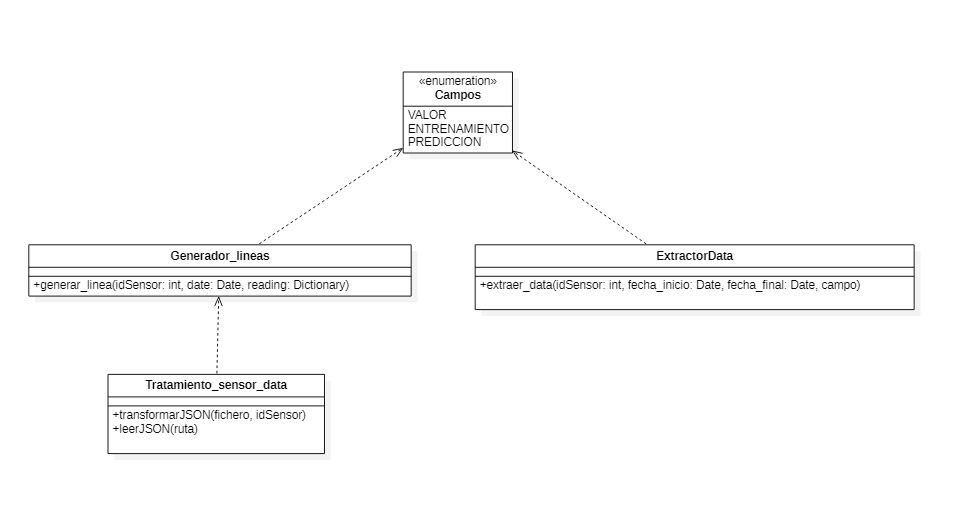
\includegraphics[width=1.1\textwidth]{img/img_diagrama_clases_utilidades.png}
	\caption{Diagrama de clases paquete Utilidades}
	\label{img_diagrama_clases_Utilidades}
\end{figure}

\newpage

\section{Diseño procedimental}
En este apartado se mostrará el funcionamiento interno del proyecto.

\subsection{Diagrama de secuencias}
Para facilitar el seguimiento de el diagrama de secuencias se ha dividido en tres, el primero muestra el proceso por el cual se obtienen los datos de PRTG \ref{img_diagrama_secuencias 1}, después se realiza el entrenamiento de los datos \ref{img_diagrama_secuencias 2} y por último se hace la predicción \ref{img_diagrama_secuencias 3}.

Los elementos coloreados hacen referencia a sistemas externos, cómo son PRTG y Elasticsearch.

\begin{figure}[!h]
	\centering
	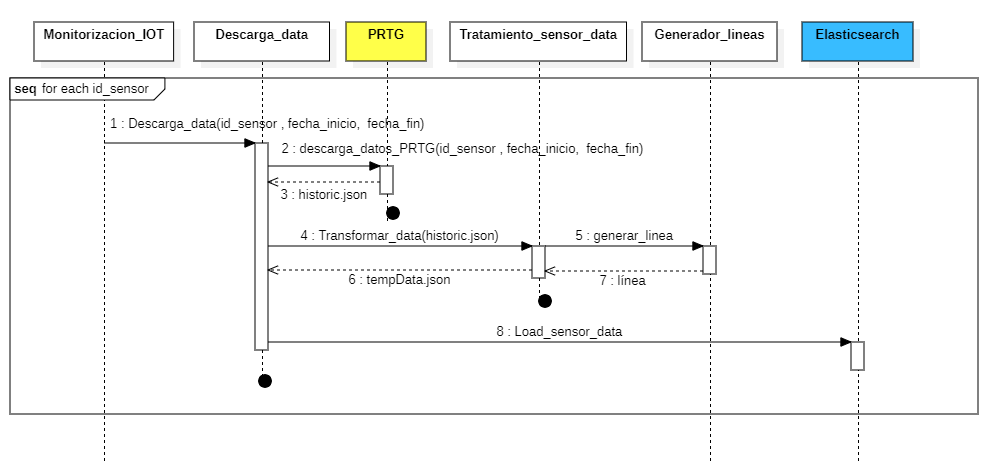
\includegraphics[width=1.1\textwidth]{img/img_diagrama_secuencias_1.png}
	\caption{Diagrama de secuencias descarga de datos}
	\label{img_diagrama_secuencias 1}
\end{figure}

\begin{figure}[!h]
	\centering
	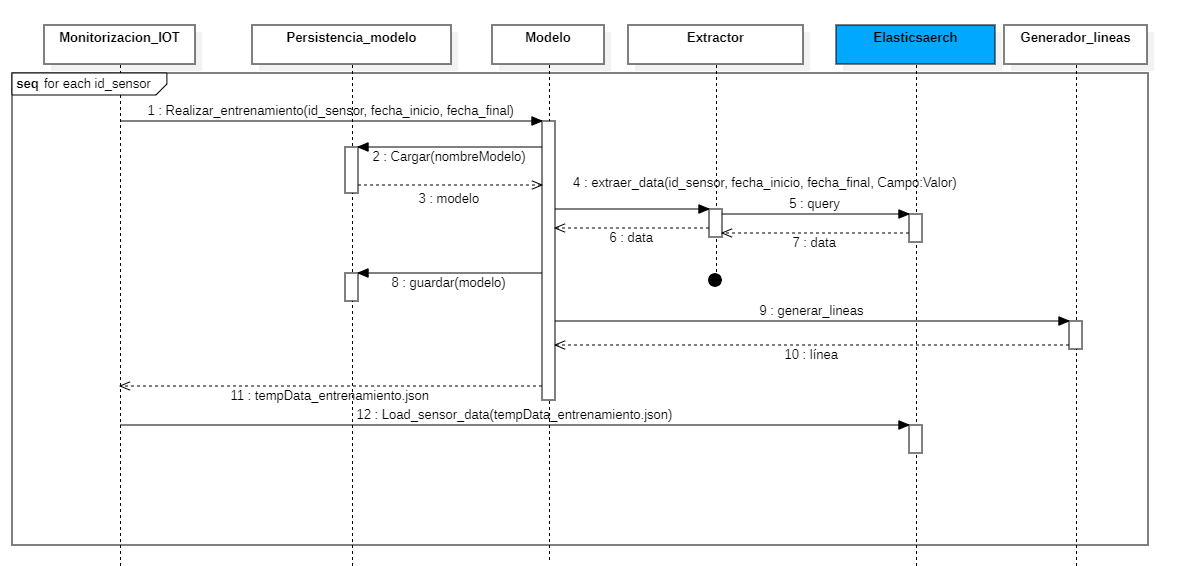
\includegraphics[width=1.1\textwidth]{img/img_diagrama_secuencias_2.png}
	\caption{Diagrama de secuencias entrenamiento}
	\label{img_diagrama_secuencias 2}
\end{figure}

\begin{figure}[!h]
	\centering
	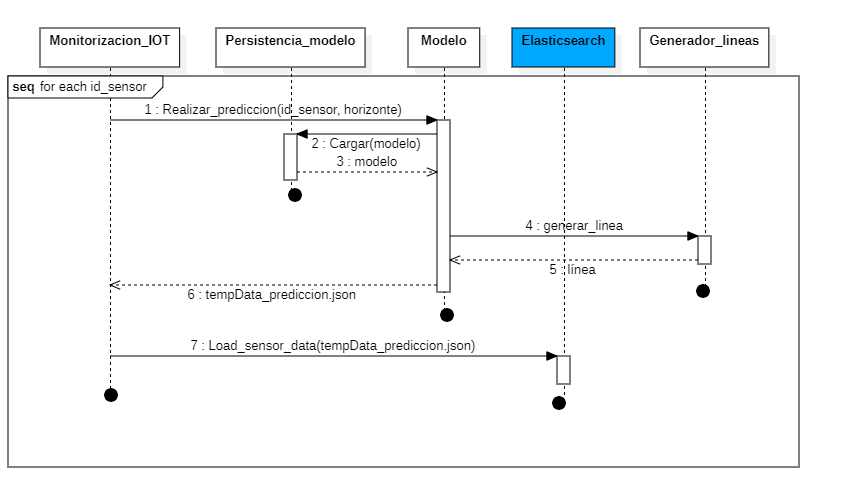
\includegraphics[width=1.1\textwidth]{img/img_diagrama_secuencias_3.png}
	\caption{Diagrama de secuencias predicción}
	\label{img_diagrama_secuencias 3}
\end{figure}
\newpage



\clearpage
\subsection{Funcionamiento de \nombrePrograma}

El núcleo del programa es el script \textit{Monitorizacion\_IOT.sh} el cual es llamado por un servicio que se repite cada X segundos. A continuación, se mostrará el pseudocódigo del script:

\noindent\fbox{
    \begin{minipage}{1\textwidth}
    \begin{algorithmic}[1]
    
        \While{True}
            \State fecha\_inicio \gets Fecha\_actual - 30 minutos $
            \State fecha\_fin \gets Fecha\_actual $
                
            \For{id\_sensor in lista\_sensores}
            
                \State Descargar\_data(id\_sensor, fecha\_inicio, fecha\_fin)
                
                \State Realizar\_entrenamiento(id\_sensor, fecha\_inicio, fecha\_fin)
                \State Load\_sensor\_datos ("tempData\_entrenamiento"" + id\_sensor + "".json")
                \State Borrar\_datos\_predicciones(id\_sensor, horizonte\_prediccion)
                \State Realizar\_predicciones(id\_sensor, fecha\_fin)
                \State Load\_sensor\_datos("tempData\_prediccion"" + id\_sensor + "".json")
                
            \EndFor
        \EndWhile
    \end{algorithmic}
    \end{minipage}
}

Pseudocódigo del script \textit{Descargar\_data.sh}, el cual es referenciado en el primer script:

\noindent\fbox{
\begin{minipage}{1\textwidth}
\begin{algorithmic}[1]

\If{fichero ""tempData"" + id\_sensor + "".json"" exist}
            \State descarga\_datos\_PRTG
            \State transformar\_datos 
            \State comparar\_ficheros
            \State Load\_sensor\_datos 
        \Else
            \State descarga\_datos\_PRTG
            \State transformar\_datos
            \State Load\_sensor\_datos
        \EndIf

\end{algorithmic}
\end{minipage}
}

\newpage
\subsection{Recolección de los datos de sensores PRTG}

Para recuperar datos históricos, PRTG permite descargarlos en diversos formatos cómo pueden ser XML, CSV o JSON, en el caso de esta aplicación, debido a la facilidad que tiene Elasticsearch con formatos JSON se decidió obtener los datos en este formato. \cite{pagina:PRTG}

Los párametros que se introducen a la llamada al comando Curl son:
\begin{itemize}
    \item \textbf{id}: el id del sensor del que se quiere descargar los históricos.
    \item \textbf{avg}(average): se pone esta variable con valor a 0 para descargar los datos en bruto.
    \item \textbf{usecaption}: se pone esta variable con valor a 1 para obtener más información del sensor y no solo la tabla de datos.
    \item \textbf{sdate}: fecha de inicio del rango
    \item \textbf{edate}: fecha de fin del rango
    \item \textbf{username}: nombre de usuario de PRTG
    \item \textbf{passhash}: passhash del usuario de PRTG
\end{itemize}


Los datos obtenidos son volcados a un fichero JSON, el cual responde al nombre historic+id\_sensor+.json


 \begin{verbatim}    
# Función que descarga datos de PRTG

# $1 : idSensor
# $2 : fecha inicio
# $3 : fecha fin
# $4 : volcado datos
function descarga_datos_PRTG(){

    curl -o "$4" $IP_PRTG'/api/historicdata.json?id='$1'
        &avg=0
        &usecaption=1
        &sdate='$2'
        &edate='$3'
        &username='$usuario_PRTG'
        &passhash='$passhash_PRTG
}
\end{verbatim}   
\caption{función del fichero 
/usr/bin/Monitorizacion\_IOT/Gestion\_datos/Descargar\_data.sh}    


\subsection{Subida de datos a Elasticsearch}
    
Para poder realizar la subida de datos a Elasticsearch de forma continua hay que configurar logstash, para ello se usa un plugin llamado Http input plugin. 

Con este plugin una aplicación puede enviar una petición http y logstash lo procesará y enviará a Elasticsearch.\cite{pagina:Http_plugin_input}

\begin{verbatim}    

input{
        http{
                id=> "sensor_data_http_input"
        }
}

filter{

        ruby {
                code => '
                    event.get("reading").each { |k, v|
                        event.set(k,v)
                    }
                    event.remove("reading")
                '
            }

}
output{

        elasticsearch{
                hosts => ["localhost:9200", "IP_Ubuntu_server:9200"]
                index => "sensor_data-%{+YYYY.MM.dd}"
        }
}

\end{verbatim}  
\caption{fichero  /etc/logstash/conf.d/logstashSensor.conf}    


Para enviar las líneas JSON con los datos a logstash se hace una petición http por línea.
\begin{verbatim}    
#!/bin/bash

IFS=$'\n'
for LINE in $(cat $1)
do
   echo $LINE
   
   curl -XPOST -u sensor_data:sensor_data --header 
   "Content-Type: application/json" 
   "http://localhost:8080/" -d ''$LINE''
done
\end{verbatim}  
\caption{fichero /usr/bin/Monitorizacion\_IOT/Gestion\_datos/Load\_sensor\_data.sh}    


    
\section{Diseño arquitectónico}

El proyecto consta de tres paquetes.

\begin{itemize}
    \item \textbf{Gestion\_data}: Este paquete se encarga de todo lo relacionado con la gestión de los datos de los sensores:. 
    \begin{itemize}
        \item Descargar los datos de PRTG.
        \item Subir datos a Elasticsearch.
        \item Descargar datos de Elasticsearch.
        \item Eliminar datos de Elasticsearch.
    \end{itemize}
    
    \item \textbf{Utilidades}: Este paquete se encarga de realizar tareas variadas como:.
        \begin{itemize}
            \item Transformar los ficheros JSON.
        \end{itemize}
    \item \textbf{Prediccion}: Este paquete se encarga de todo lo relacionado con el entrenamiento y la predicción de los sensores:
        \begin{itemize}
            \item Entrenar el modelo.
            \item Realizar la predicción.
            \item Crear modelos.
        \end{itemize}
\end{itemize}

\clearpage

\begin{figure}[h]
	\centering
	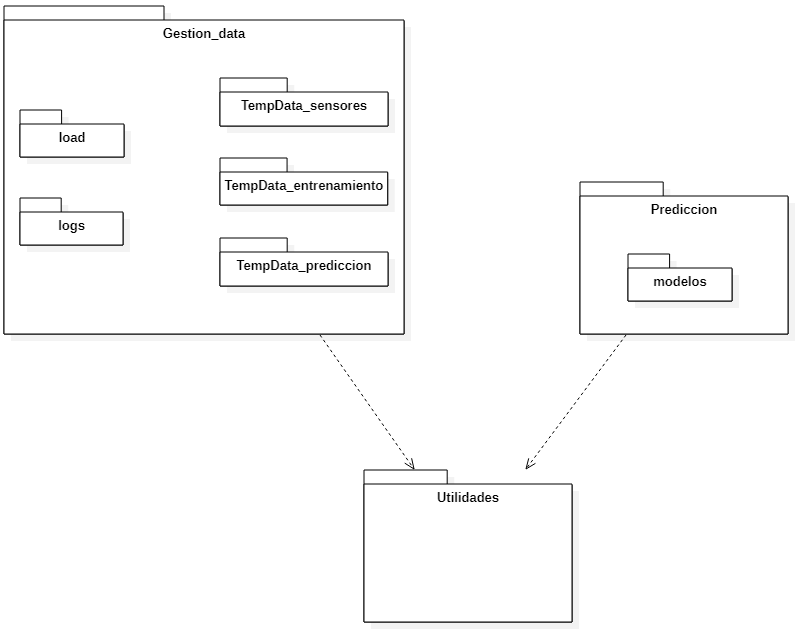
\includegraphics[width=1.0\textwidth]{img/img_diagrama_paquetes.png}
	\caption{Diagrama de paquetes}
	\label{img_diagrama_paquetes}
\end{figure}

Para facilitar el entendimiento de la topología tanto del hardware cómo del software se presenta el siguiente diagrama de despliegue \ref{img_diagrama_despliegue}. En el se pueden observar los dos sistemas: ubuntu server, albergando Elasticsearch y \nombrePrograma y Windows 10 cuya única función es albergar PRTG.

\begin{figure}[h]
	\centering
	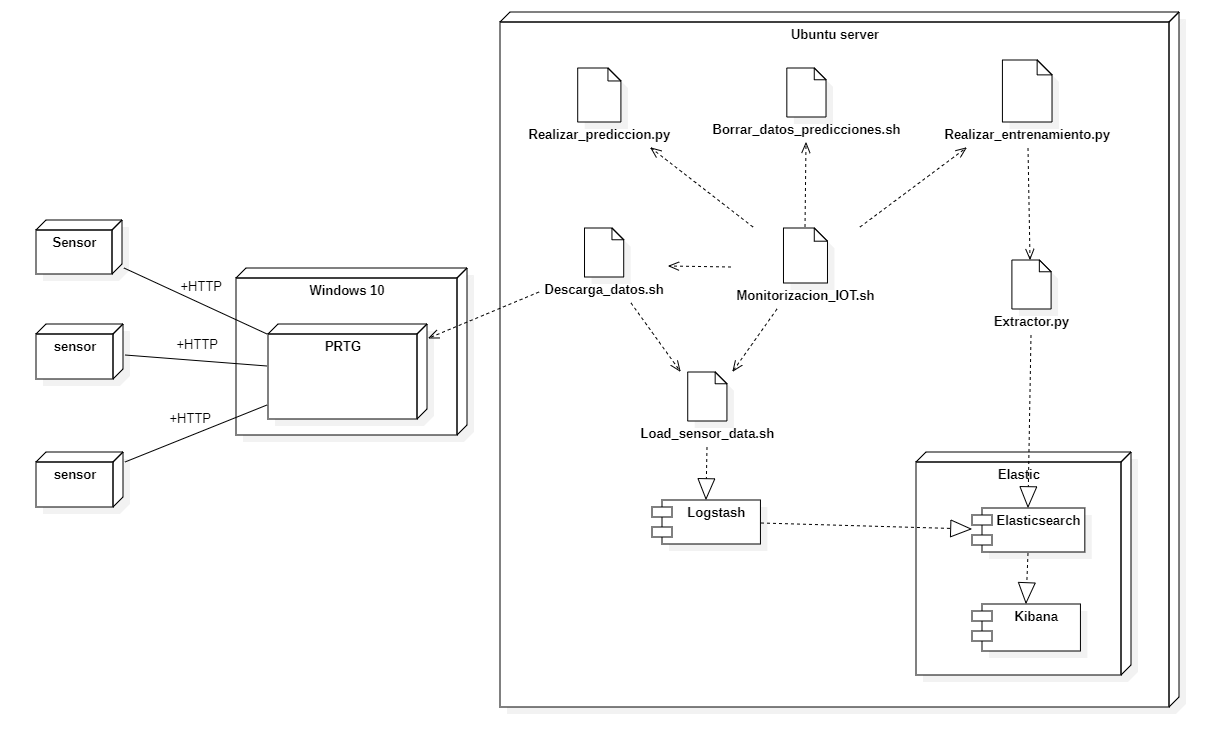
\includegraphics[width=1.0\textwidth]{img/img_diagrama_despliegue.png}
	\caption{Diagrama de despliegue}
	\label{img_diagrama_despliegue}
\end{figure}